\section{Use Case}

% Introductory slide

\begin{frame}{Persona}
	\begin{columns}
		
		\begin{column}{0.5\textwidth}
			\centering
			
\includegraphics[width=0.6\linewidth]{images/paolo.png}			
		\end{column}
		
		\begin{column}{0.5\textwidth}
			
			\begin{itemize}
				\item Paolo Dibali
				\item Age 27
				\item Video Game Designer 
				\item Paolo wants to create his video game
			\end{itemize}
			
		\end{column}
		
	\end{columns}
	
	\vspace{0.5cm}
	
	\begin{itemize}
		\item Non-Player Characters (NPCs) approaches:
		\begin{itemize}
			\item Handcrafted rules 
			\item Reinforcement Learning (RL)
		\end{itemize}
	\end{itemize}
	
\end{frame}

\begin{frame}
\frametitle{Video games and AI}

	\begin{itemize}
		\item RL is used in video games to create NPCs
	\end{itemize}
	
	
	\begin{columns}
		\begin{column}{0.5\textwidth}
			
			\begin{itemize}
				\item Two problems:
				
				\begin{itemize}
					\item NPCs with super-human abilities
					\item NPCs with predictable behavior
				\end{itemize}
				
			\end{itemize}
			
		\end{column}
		\begin{column}{0.5\textwidth}
			\centering
			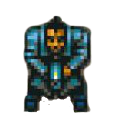
\includegraphics[width=0.4\linewidth]{images/npc2.png}		
		\end{column}
		
	\end{columns}
	
	\vspace{0.5cm}
	
	\begin{itemize}
		\item<2-> \textbf{Solution:} Paolo can control the agent behavior $\Rightarrow$ IRL %Use in the agent train a human control
	\end{itemize}

\end{frame}

% Reinforcement Learning slide

\begin{frame}
	\frametitle{Reinforcement Learning vs Inverse Reinforcement Learning}
	
 	\begin{columns}
		\begin{column}{0.5\textwidth}
			
			\begin{itemize}
				\item<1-> RL agent takes environments rewards
				\item<2-> The agent learns the behavior through trial-and-error mechanism
			\end{itemize}
			
		\end{column}
		\begin{column}{0.5\textwidth}
			\begin{itemize}
				\item<1-> IRL agent receives rewards from a Reward Model
				\item<2-> The user controls the agent behavior with preference feedback 
			\end{itemize}			
		\end{column}
		
	\end{columns}
	\vspace{1cm}
	\centering
	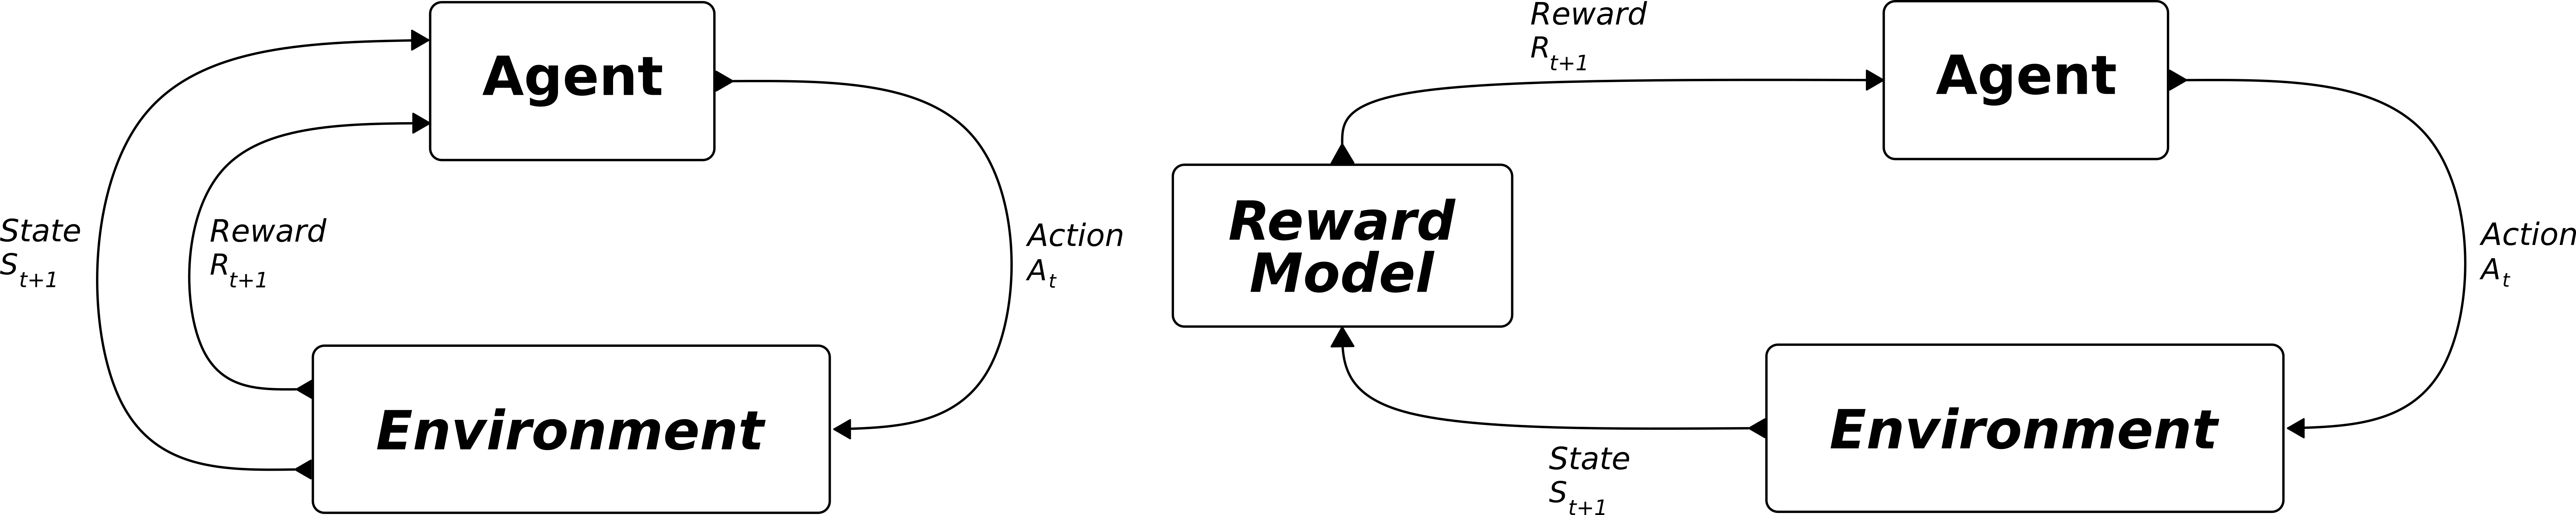
\includegraphics[width=1\linewidth]{images/IRL+RL.png}

\end{frame}


\begin{comment}	
\begin{columns}
\begin{column}{0.5cm\textwidth}
\begin{itemize}
\item Reinforcement Learning is the science of making
optimal decisions using experiences
\item  Find an optimal behavior
strategy for the agent to obtain optimal rewards
\end{itemize}
\end{column}
\begin{column}{0.5cm\textwidth}
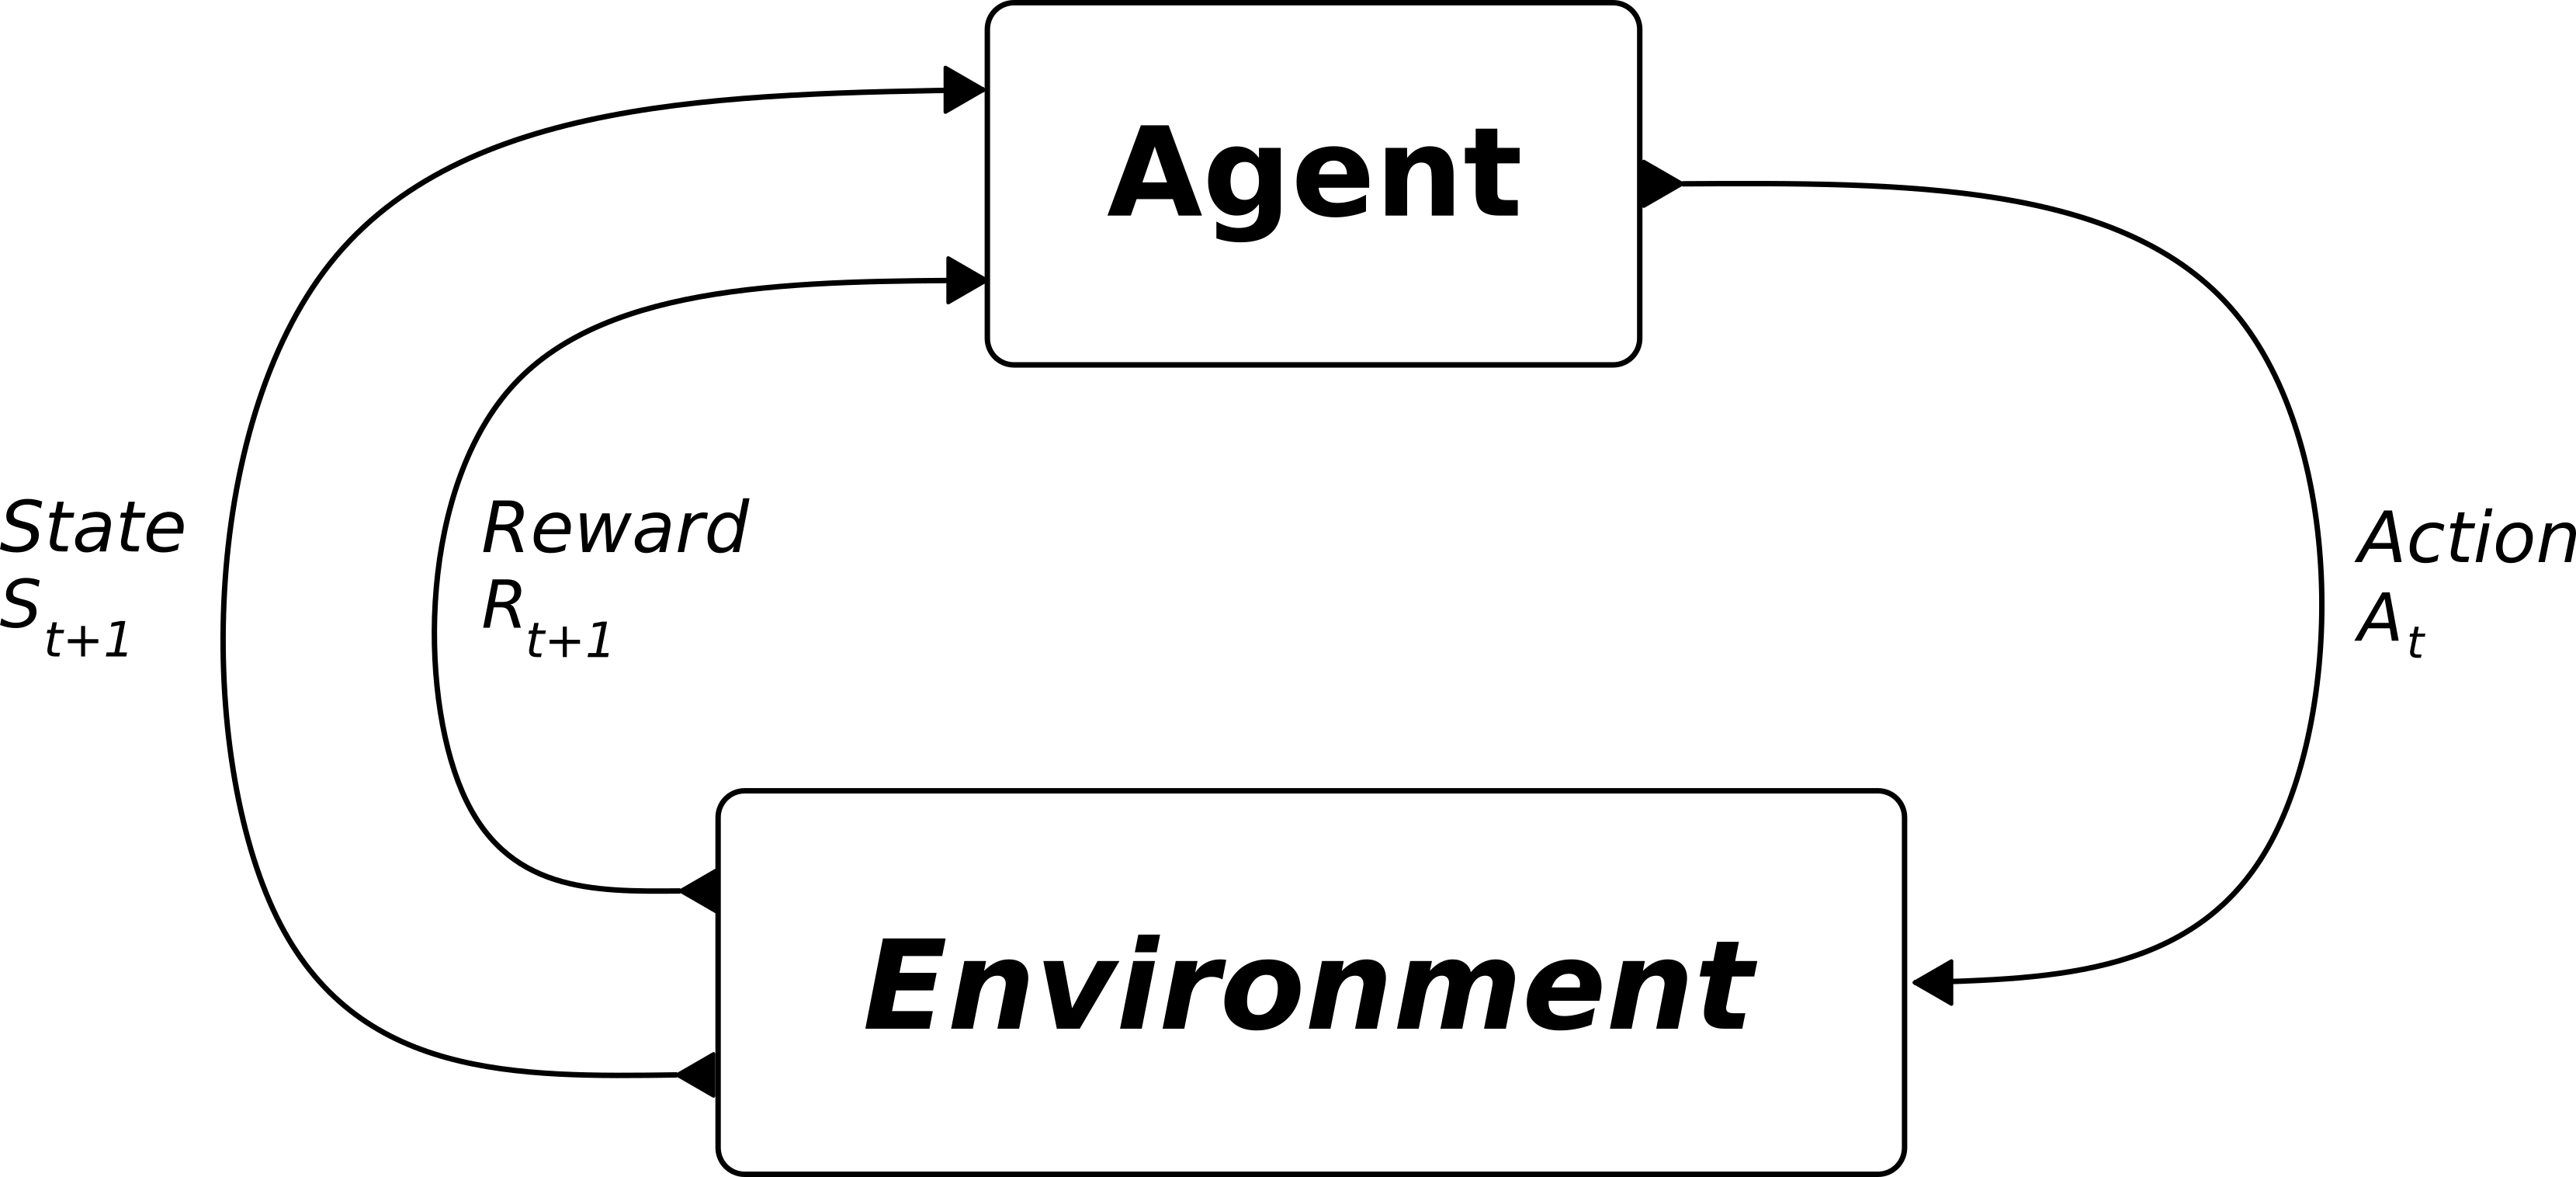
\includegraphics[width=0.60\linewidth]{images/RL.png}
\end{column}
\end{columns}

\begin{columns}<2->
\begin{column}{0.5cm\textwidth}
\begin{itemize}
\item The agent does not receive the reward from environment
\item A human in the loop communicates to the agent his intentions 
\end{itemize}
\end{column}
\begin{column}{0.5cm\textwidth}
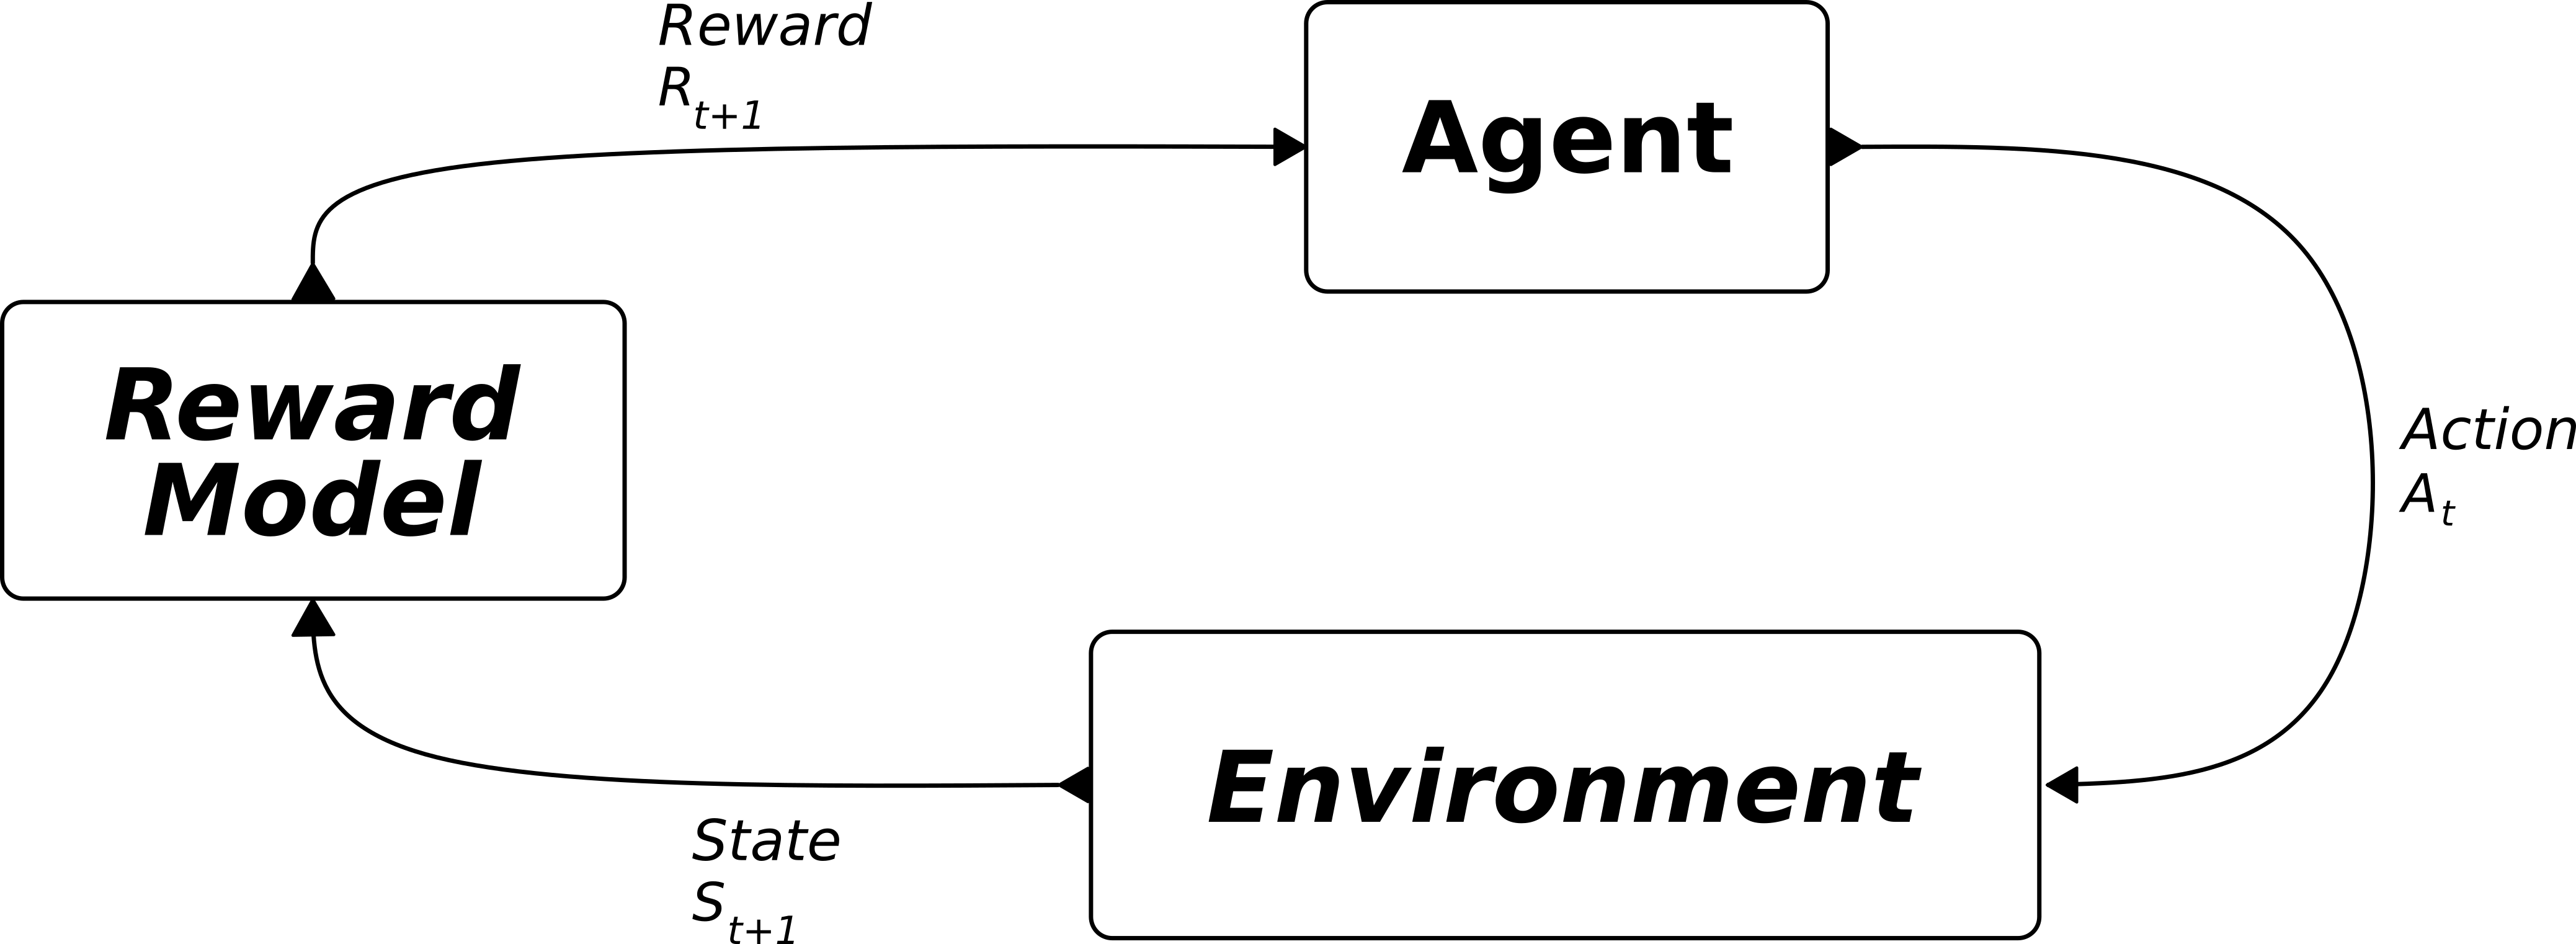
\includegraphics[width=0.60\linewidth]{images/IRL.png}
\end{column}
\end{columns}

	\begin{itemize}
	\item Reinforcement Learning is the science of making
	optimal decisions using experiences
	\item  Find an optimal behavior
	strategy for the agent to obtain optimal rewards
	\end{itemize}
	
	\begin{figure}
	\centering
	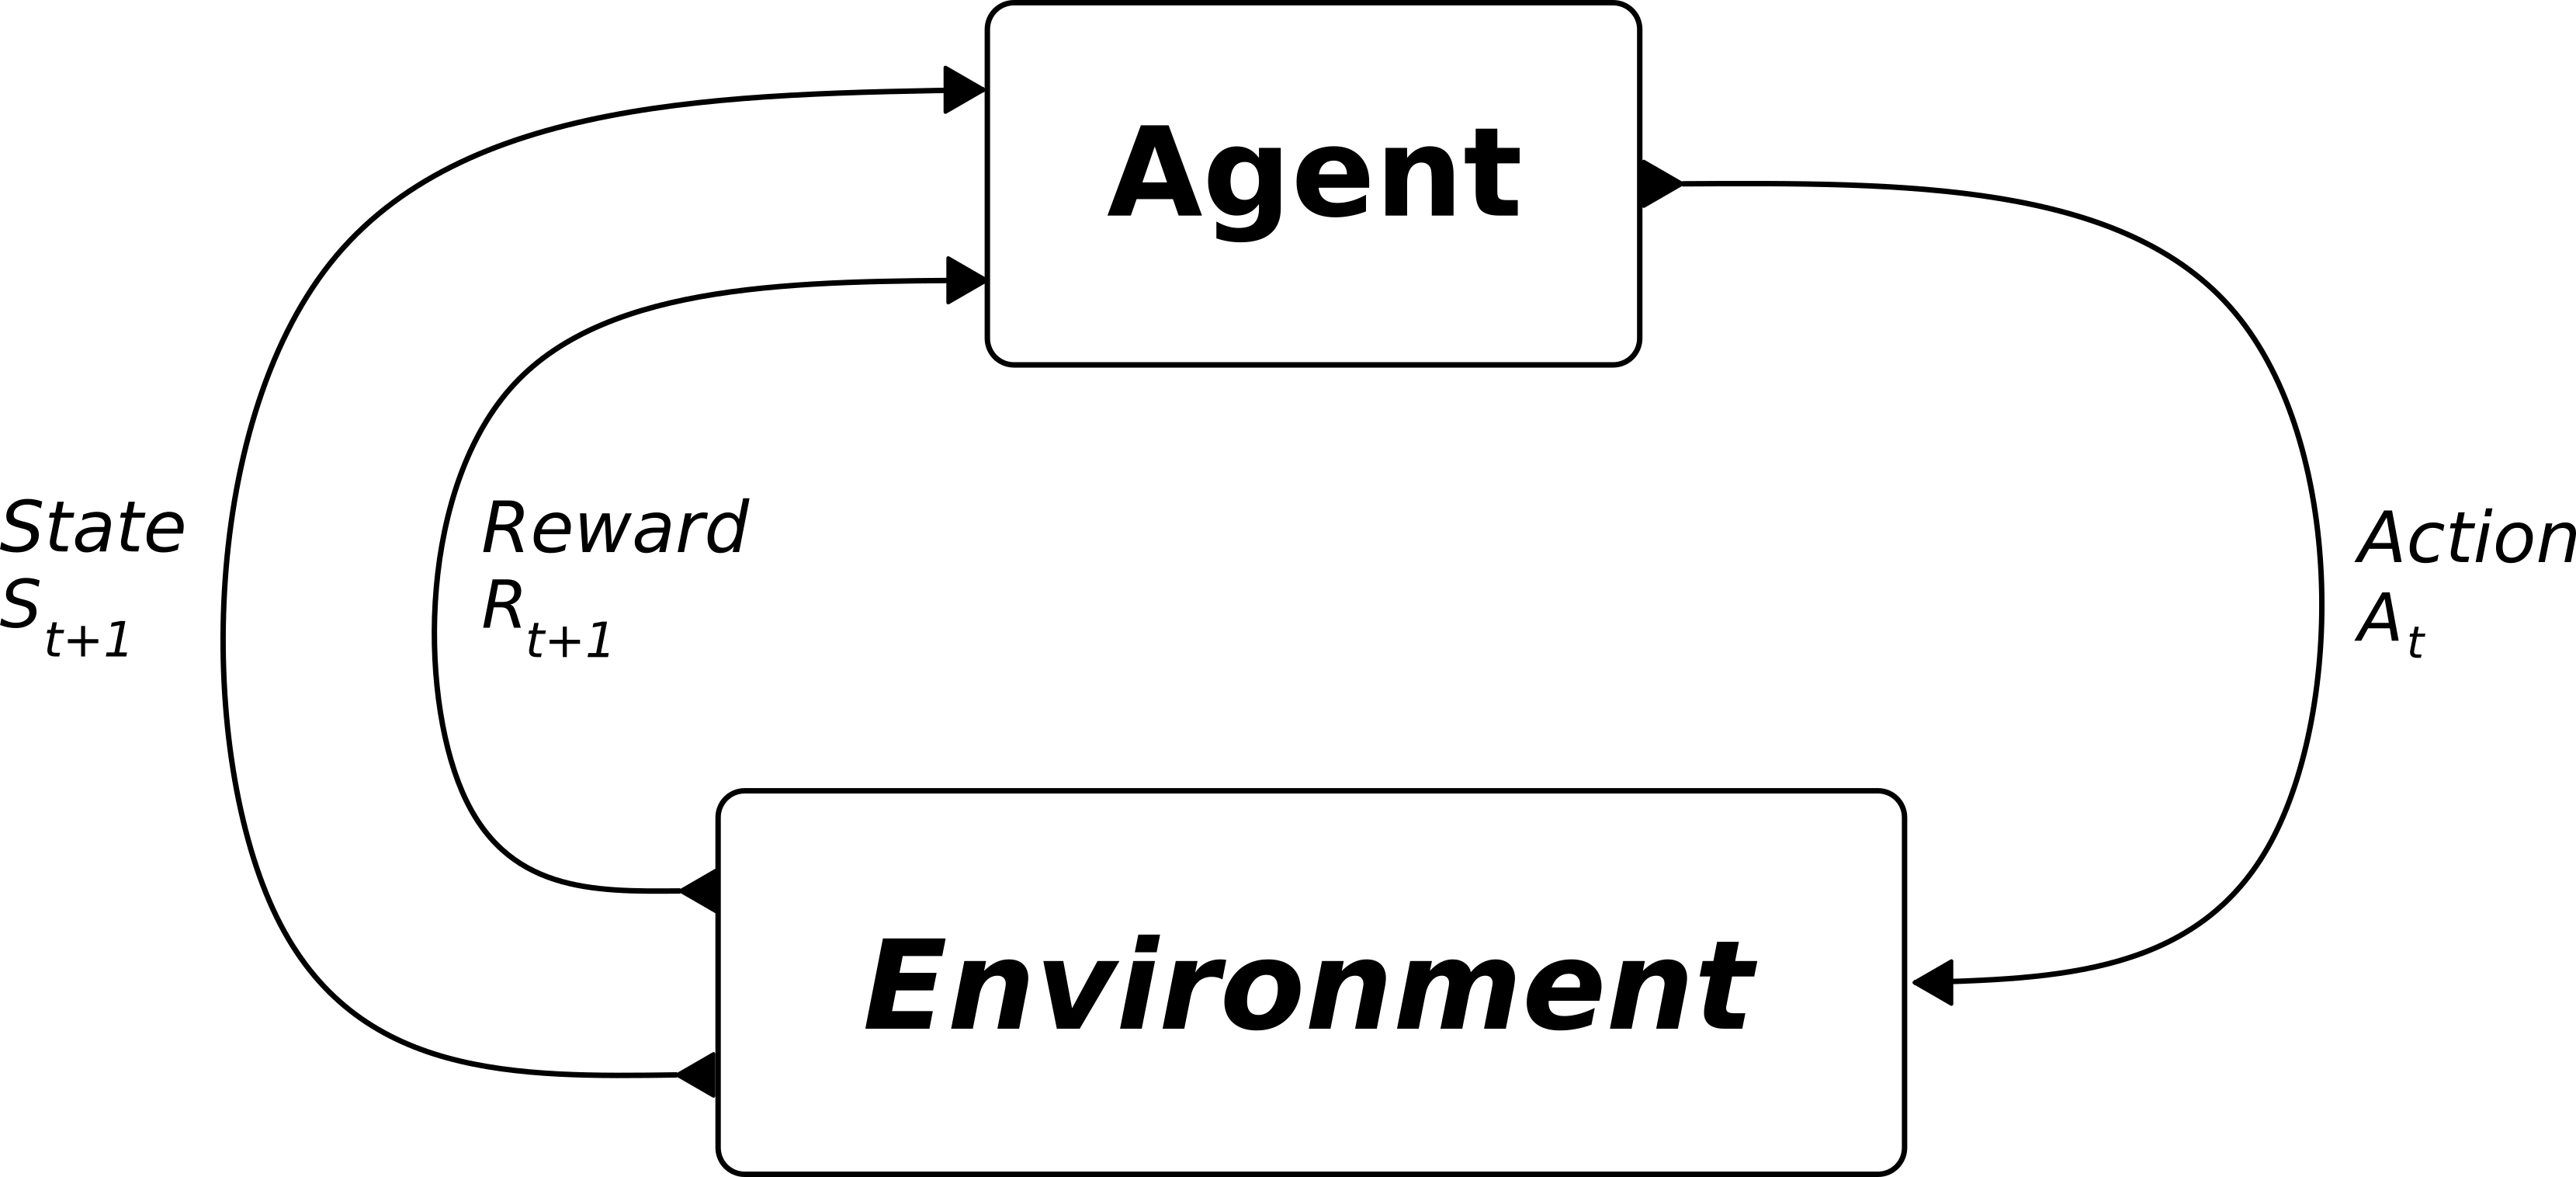
\includegraphics[width=0.60\linewidth]{images/RL.png}
	\end{figure}
	
	\end{frame}
	
	% Inverse Reinforcement Learning slide
	\begin{frame}
	\frametitle{Inverse Reinforcement Learning}
	
	\begin{itemize}
	\item The agent does not receive the reward from environment
	\item A human in the loop communicates to the agent his intentions 
	\end{itemize}
	
	\begin{figure}
	\centering
	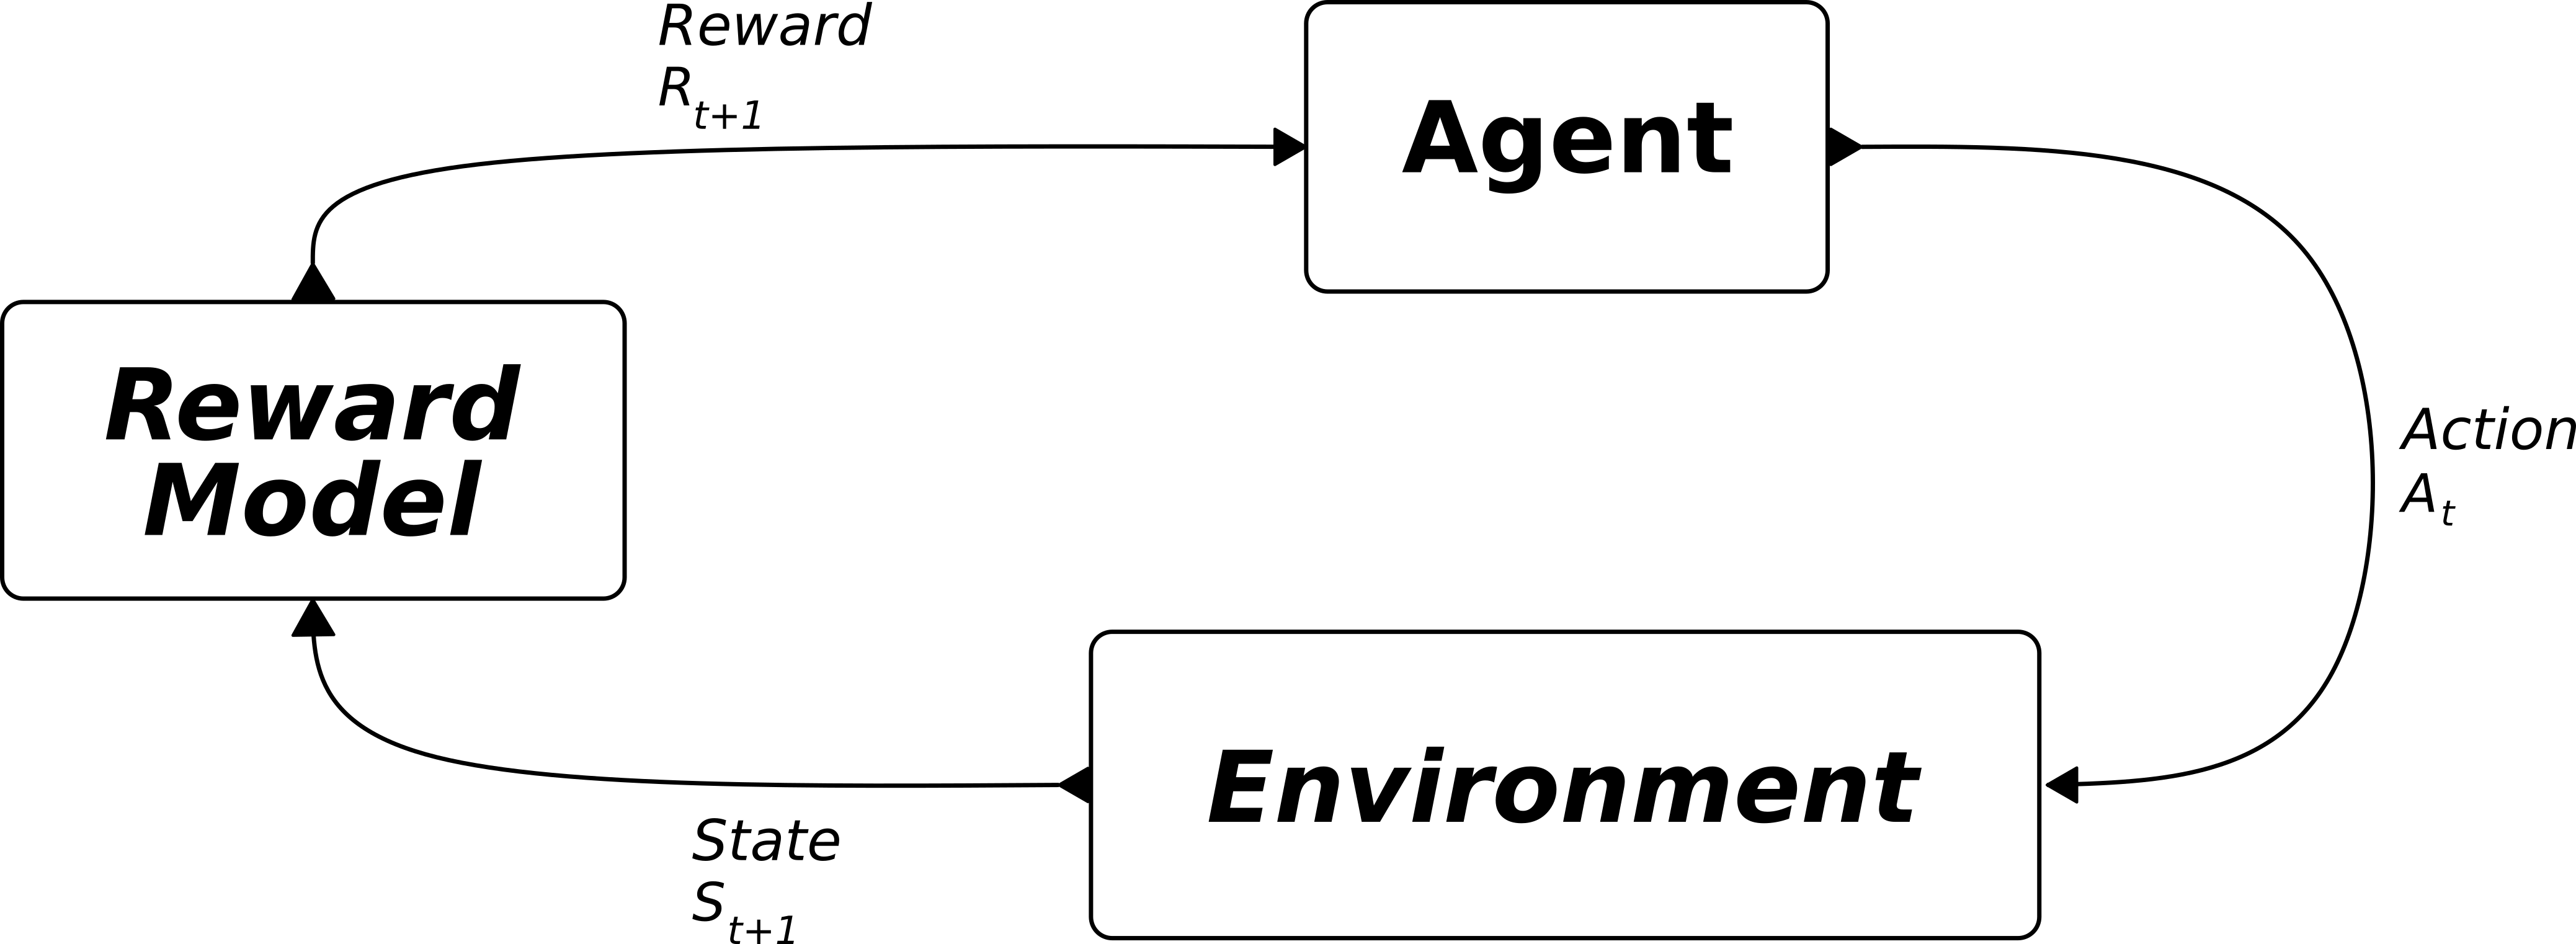
\includegraphics[width=0.60\linewidth]{images/IRL.png}
	\end{figure}
	
	\end{frame}
	
\end{comment}

